% This is samplepaper.tex, a sample chapter demonstrating the
% LLNCS macro package for Springer Computer Science proceedings;
% Version 2.21 of 2022/01/12
%
\documentclass[runningheads]{llncs}
\usepackage{xcolor}
\usepackage{setspace}
\usepackage[T1]{fontenc}
% T1 fonts will be used to generate the final print and online PDFs,
% so please use T1 fonts in your manuscript whenever possible.
% Other font encondings may result in incorrect characters.
\newcommand{\link}[2]{\href{#1}{\color{blue}\underline{\smash{#2}}}}
\usepackage{hyperref}
\usepackage{graphicx}
% Used for displaying a sample figure. If possible, figure files should
% be included in EPS format.
%
% If you use the hyperref package, please uncomment the following two lines
% to display URLs in blue roman font according to Springer's eBook style:
%\usepackage{color}
%\renewcommand\UrlFont{\color{blue}\rmfamily}
%\urlstyle{rm}
%
\begin{document}
%
\title{2D Sample Holder Building Instructions}
%
%\titlerunning{Abbreviated paper title}
% If the paper title is too long for the running head, you can set
% an abbreviated paper title here
%
\author{Filippo Armando Govi \inst{1} \\~\\ Supervisor: Sanli Faez \inst{2}}

\institute{Utrecht University
\and
Utrecht University, Nanophotonics group}
%
\maketitle              % typeset the header of the contribution
%
%
%
%
\doublespacing

\section*{Introduction}

The Flamingo microscope requires a laser to be shined to the sample at a reflection angle from the side of the camera. For this to be possible in a compact and easy to set-up build, one must a sample holder with a hollow center, so that images of the sample can be taken. At the same time, in order to be able to see different parts of the sample accurately, one needs a sample holder that moves in the x and y directions with a central hole. Since we could not find any such sample holders of appropriate size and cost, we decided to design one ourselves. 

The current design of the 2D Sample Holder was designed with ease of manifacturing in mind, and is easily modifiable to fit the desired specifications for other microscopes thanks to its parametric design in Fusion 360. The 2D-moving stage has been designed to give approximately 30 mm of travel in both the x and y directions. This allows the user to fully explore each sample.

\section*{Sample Holder Design}

The 2D stage consists of three components printed in place with the use of a 3D printer. The outer component, shown in figure 1, has inserts along its vertical axis that the inner component (figure 2) slots in with its rails. A square nut is inserted during the 3D print inside the center horse-shoe bend in the inner component. Then the inner component can be moved along the vertical axis by placing an M3 bolt through the hole in the outer component followed by two nuts locked against each other so that as the bolt spins in place it moves the inner stage. Similarly, the inner stage has rails in the horizontal orientation and a square nut dropped in its left side. This allows us to move the inner component horizontally in the same way. In addition, it is possible to see a window in the side of the outer component, which has been carefully designed to allow access to the bolt responsible for the inner stage's horizontal movement through the stage's entire vertical range of motion. The center of the sample holder is hollow with four square protrusions where M3 square nuts should be inserted. This allows the user to screw in plaques that will hold the sample in place.

It is easy to notice that the outer walls of the sample holder are taller than its inner island. That is the case to ensure that the laser going through the microscope's Olympus stage does not interfere with the stage. 

\begin{figure}[h]
    \centering
    \begin{minipage}[b]{0.45\textwidth}
        \centering
        \includegraphics[width=\textwidth]{images/stage_outer_rim.png} % Replace with your image filename
        \caption{Outer Walls Sample Holder}
    \end{minipage}
    \hfill
    \begin{minipage}[b]{0.45\textwidth}
        \centering
        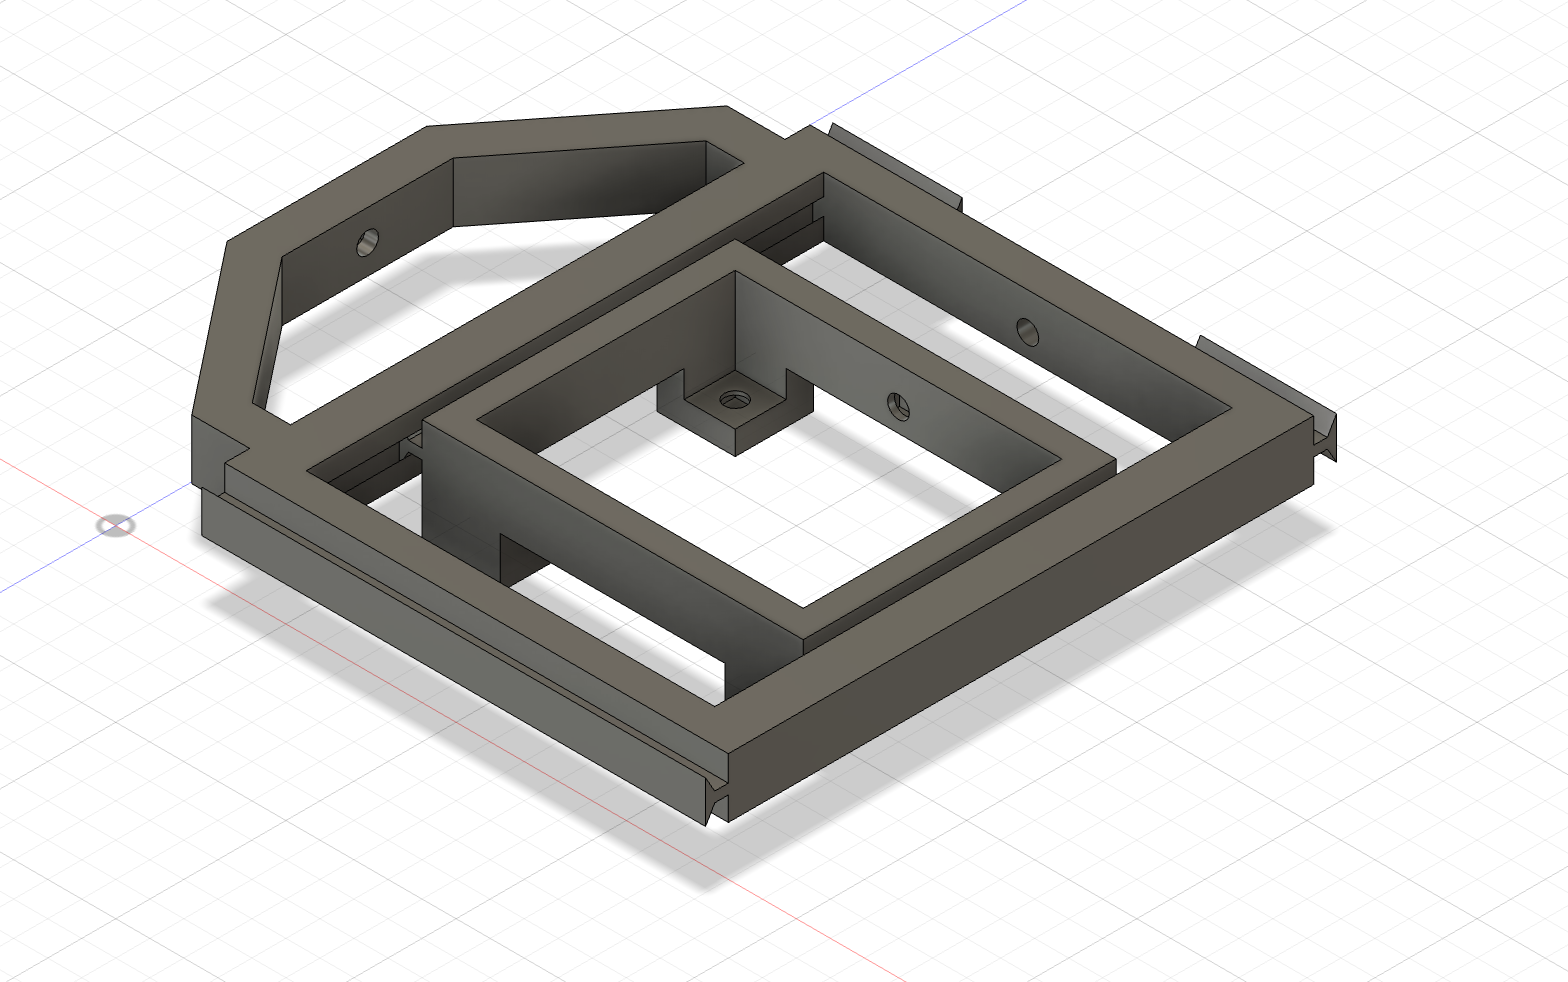
\includegraphics[width=\textwidth]{images/inner_stage.png} 
        \caption{Inner Island Sample Holder}
    \end{minipage}
\end{figure}

\section*{Print Settings}

We suggest printing the stage in tough PLA as it allows for a cleaner print of the rails, which are printed in place, hence allowing the stage to have minimal z-fluctuations as the sample is moved. The increased z-stability allows the microscope to remain focused as the sample is moved, which enables the user to more easily explore the sample. It is also advisable to print the design with a 2-layer raft beneath the sample holder, with the top of the sample holder facing the print plate as shown in figure 3.

FIG3

We suggest printing the stage using a 0.25mm nozzle heated at 205 degrees Celsius, enabling organic supports exclusively (meaning supports that start from the print plate and arch into parts of the design to be supported). This will prevent supports from being printed inside the sample holder's rails system, which would make their removal complicated and scarring of the rail system likely. This would cause increased friction in the rail system and increase the likelihood of the system jamming during use. In addition, the 3D printer will likely want to support the four square protrusions in the stage's inner island, as shown in figure 4. It is necessary to block the printer from building supports inside these square protrusions so that the four square M3 nuts can be placed inside them.

FIG 4


Lastly, since the stage is supposed to have six square nuts; five in the inner stage and one in the center of the horse-shoe bend in the inner rim of the stage as shown in figure 4, the user should pause the print at the layer right before the nut-holes are covered by the 3D printer and place the nuts in the print. Four of the M3 nuts should be placed in the squares protruding in the inner perimeter of the sample holder, these will allow the user to secure 

Notice that the hole in the inner part of the stage is lower than the one in the horseshoe bend, hence two pauses will be necessary.

\begin{figure}[h]
    \centering
    \begin{minipage}[b]{0.45\textwidth}
        \centering
        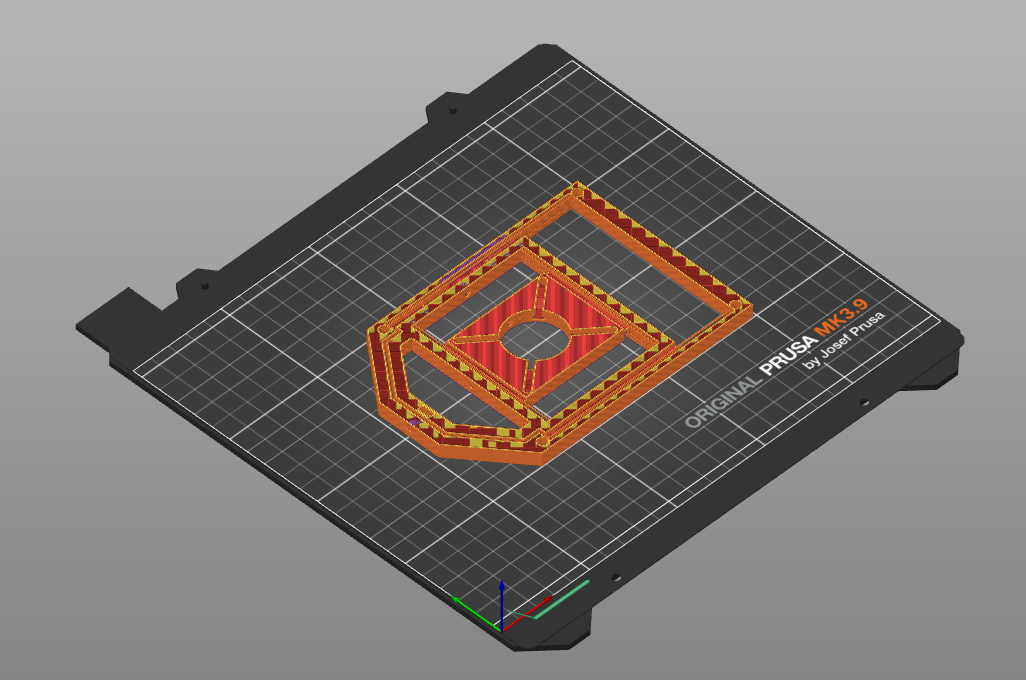
\includegraphics[width=\textwidth]{images/front_nut_3d_print_render.png} % Replace with your image filename
        \caption{Front Nut print pause}
    \end{minipage}
    \hfill
    \begin{minipage}[b]{0.47\textwidth}
        \centering
        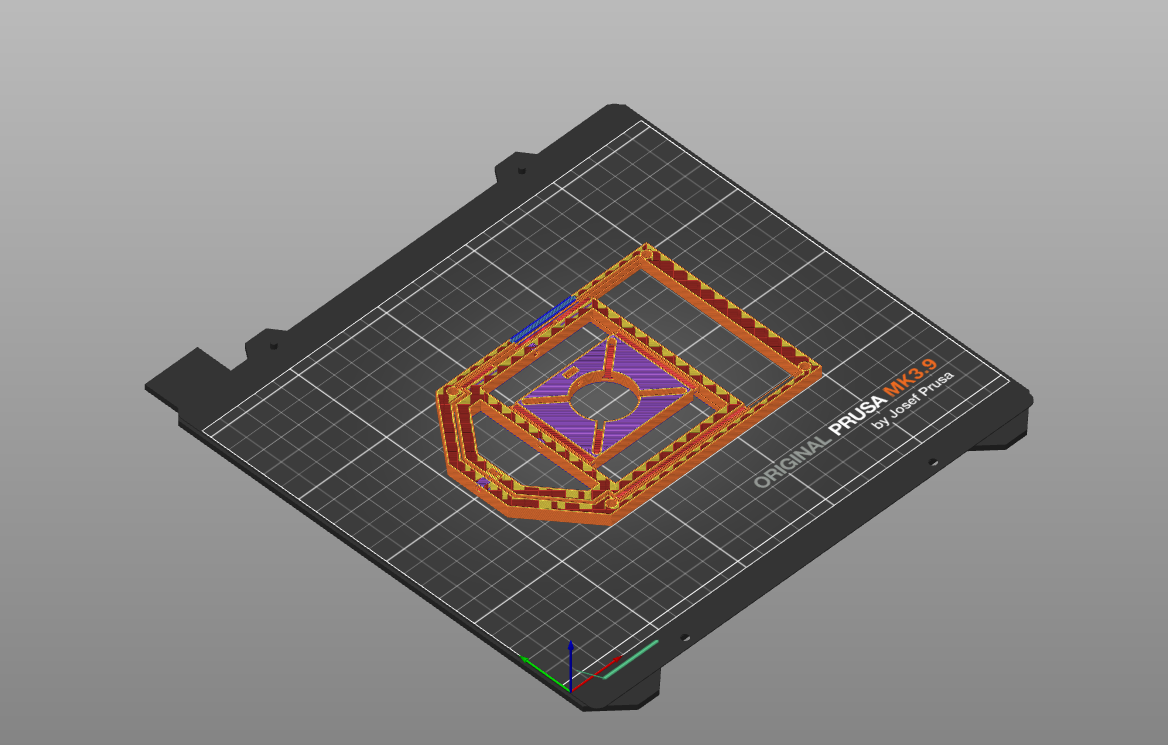
\includegraphics[width=\textwidth]{images/side_nut_3d_print_render.png} 
        \caption{Side Nut print pause}
    \end{minipage}
\end{figure}

\section*{Assembling the Sample Holder}

Once the sample holder is done printing, the x-y moving sample holder is almost ready. To complete it, you will need: four M3 nuts, one M3 bolt 36mm long, one M3 bolt 42mm long, four M2.5 bolts 15mm long, four M2.5 nuts.

Place the longer M3 bolt in the outermost front hole of the stage (on the horseshoe bend) and thread the two nuts on it. If you have an M3 bolt longer than 42mm, you should thread two nuts on the bolt before inserting it in the outermost hole and then tighten them to each other using pliers to ensure that the length by which the M3 bolt is protruding in the stage is 30mm. Then you need to lock the two nuts inside the first hole of the stage against each other as close to the outermost hole in the stage as possible but not so close that the bolt has difficulty spinning. You should repeat the same procedue for the shorter bolt in the side of the stage. The assembled bolts are shown in figures 5 and 6.

\begin{figure}[h]
    \centering
    \begin{minipage}[b]{0.45\textwidth}
        \centering
        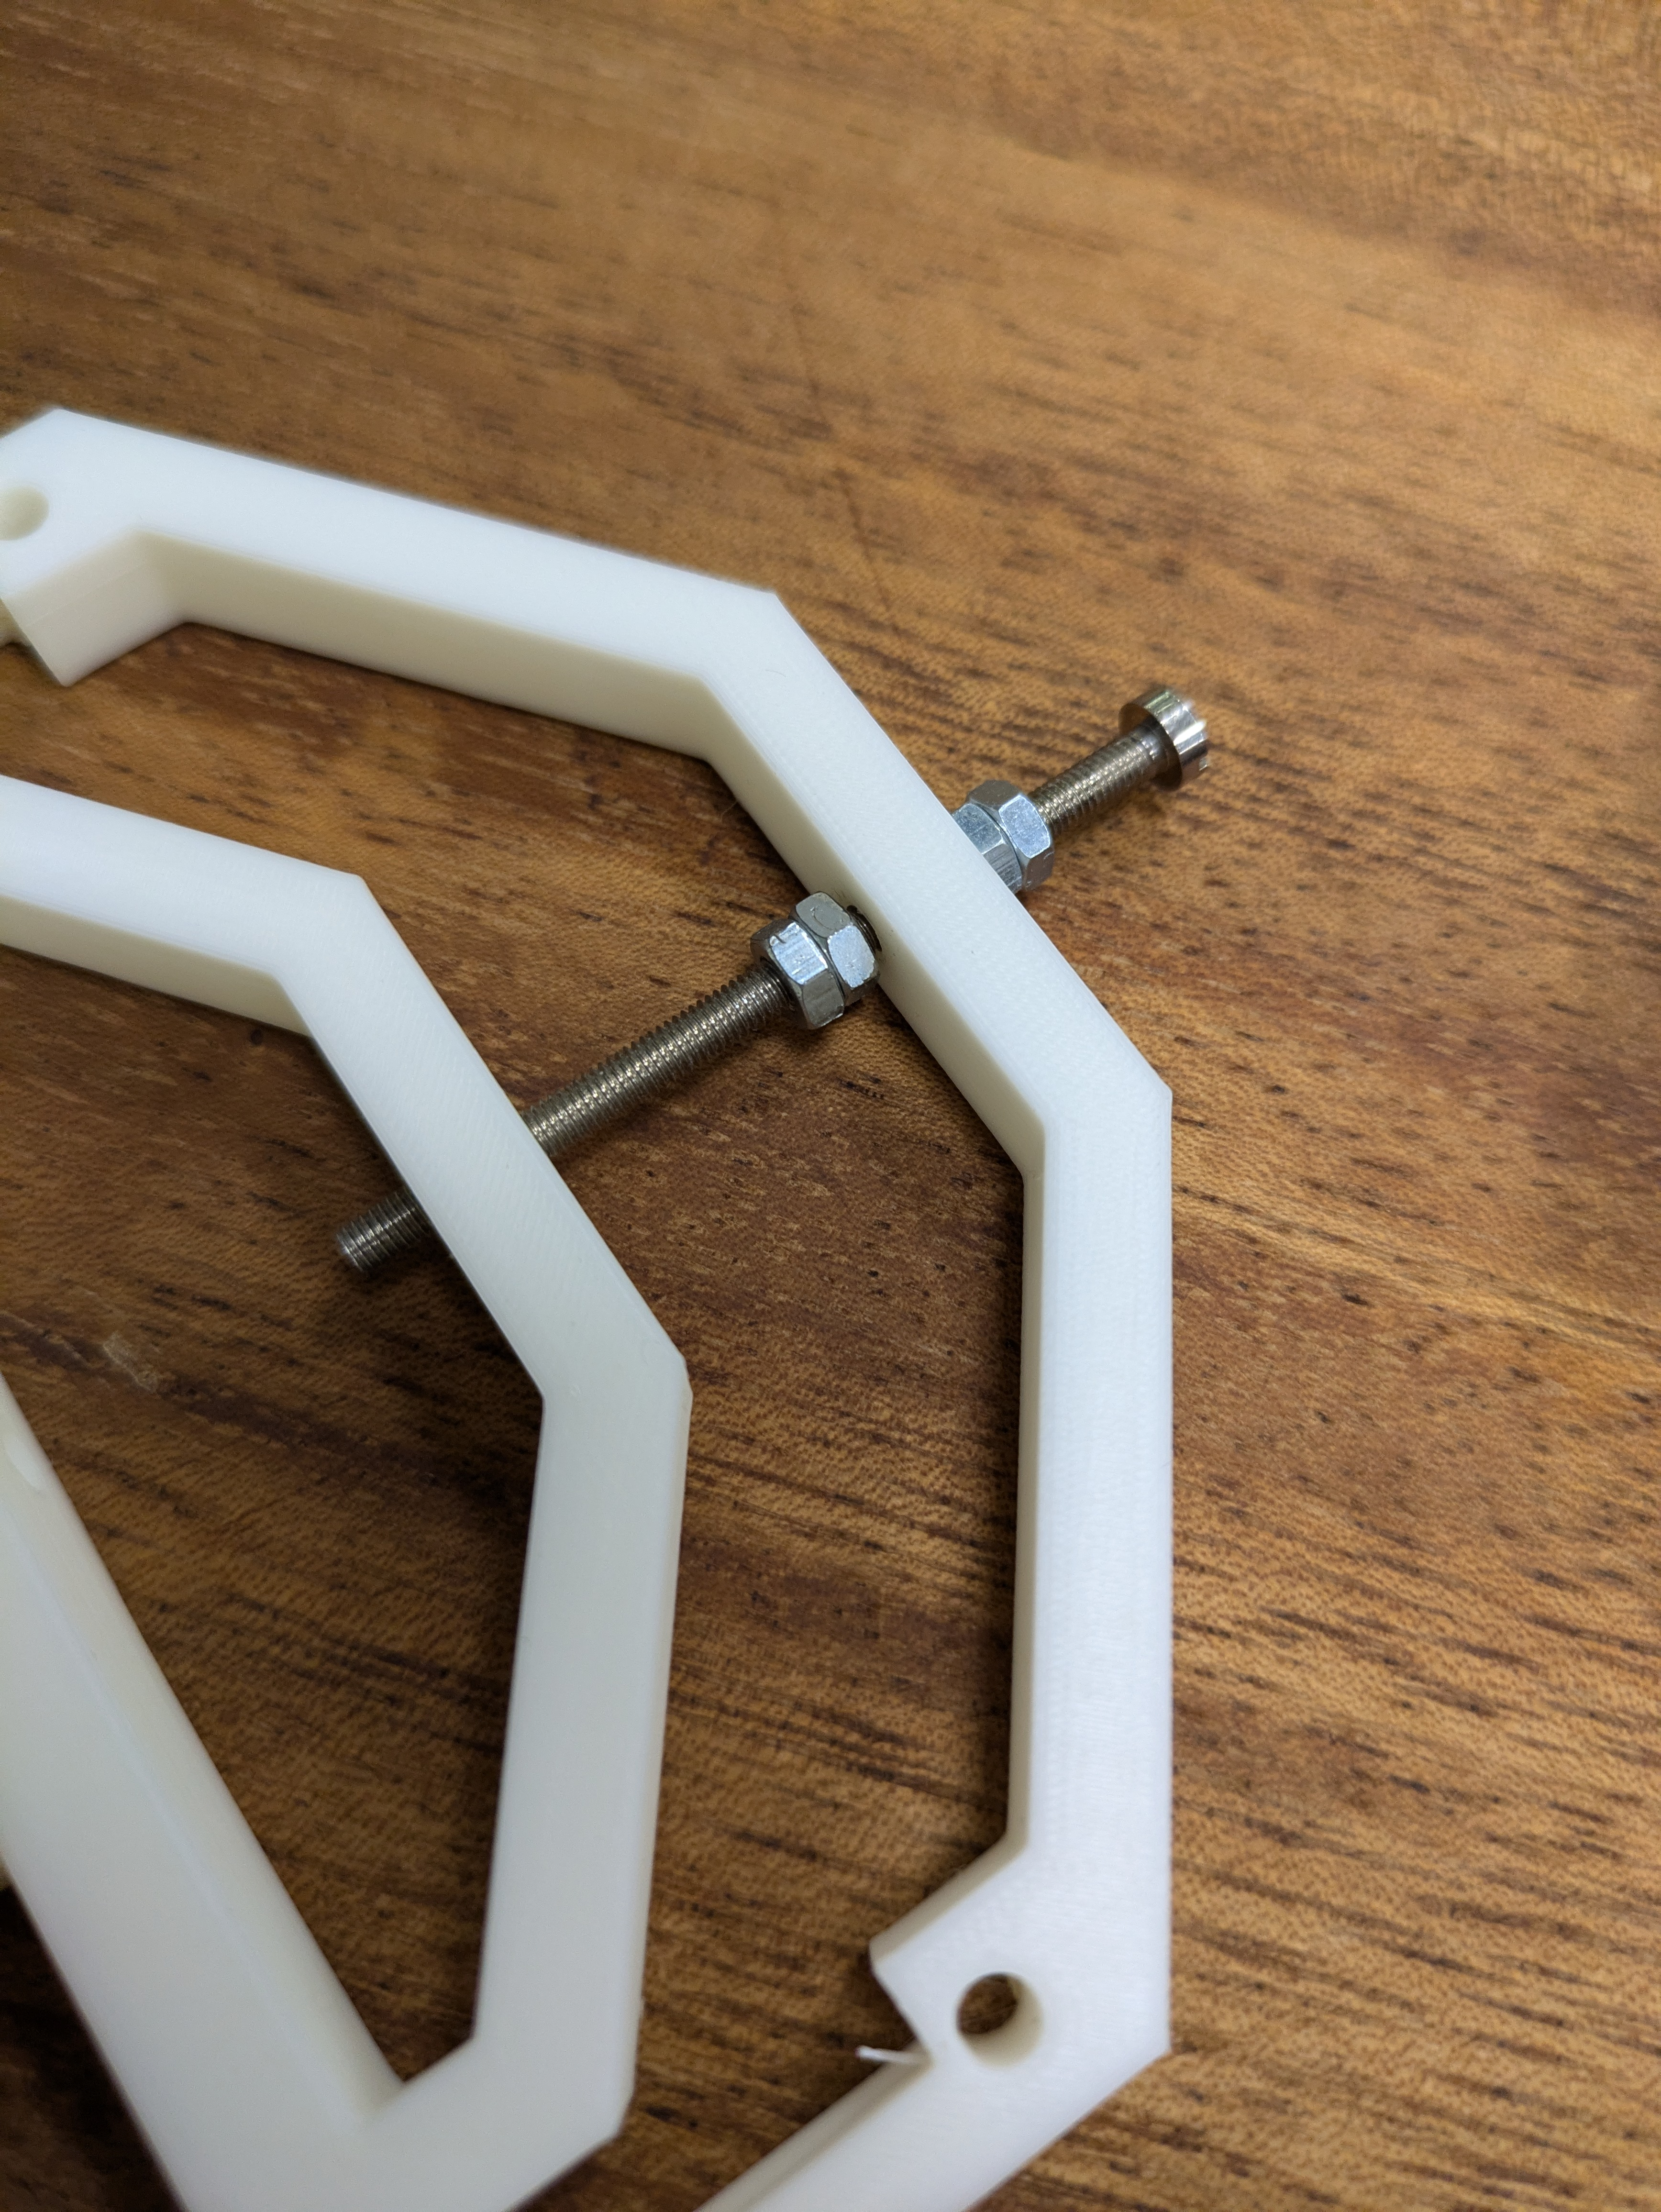
\includegraphics[width=\textwidth]{images/front_nut.jpg} % Replace with your image filename
        \caption{Properly Installed Front Nut }
    \end{minipage}
    \hfill
    \begin{minipage}[b]{0.45\textwidth}
        \centering
        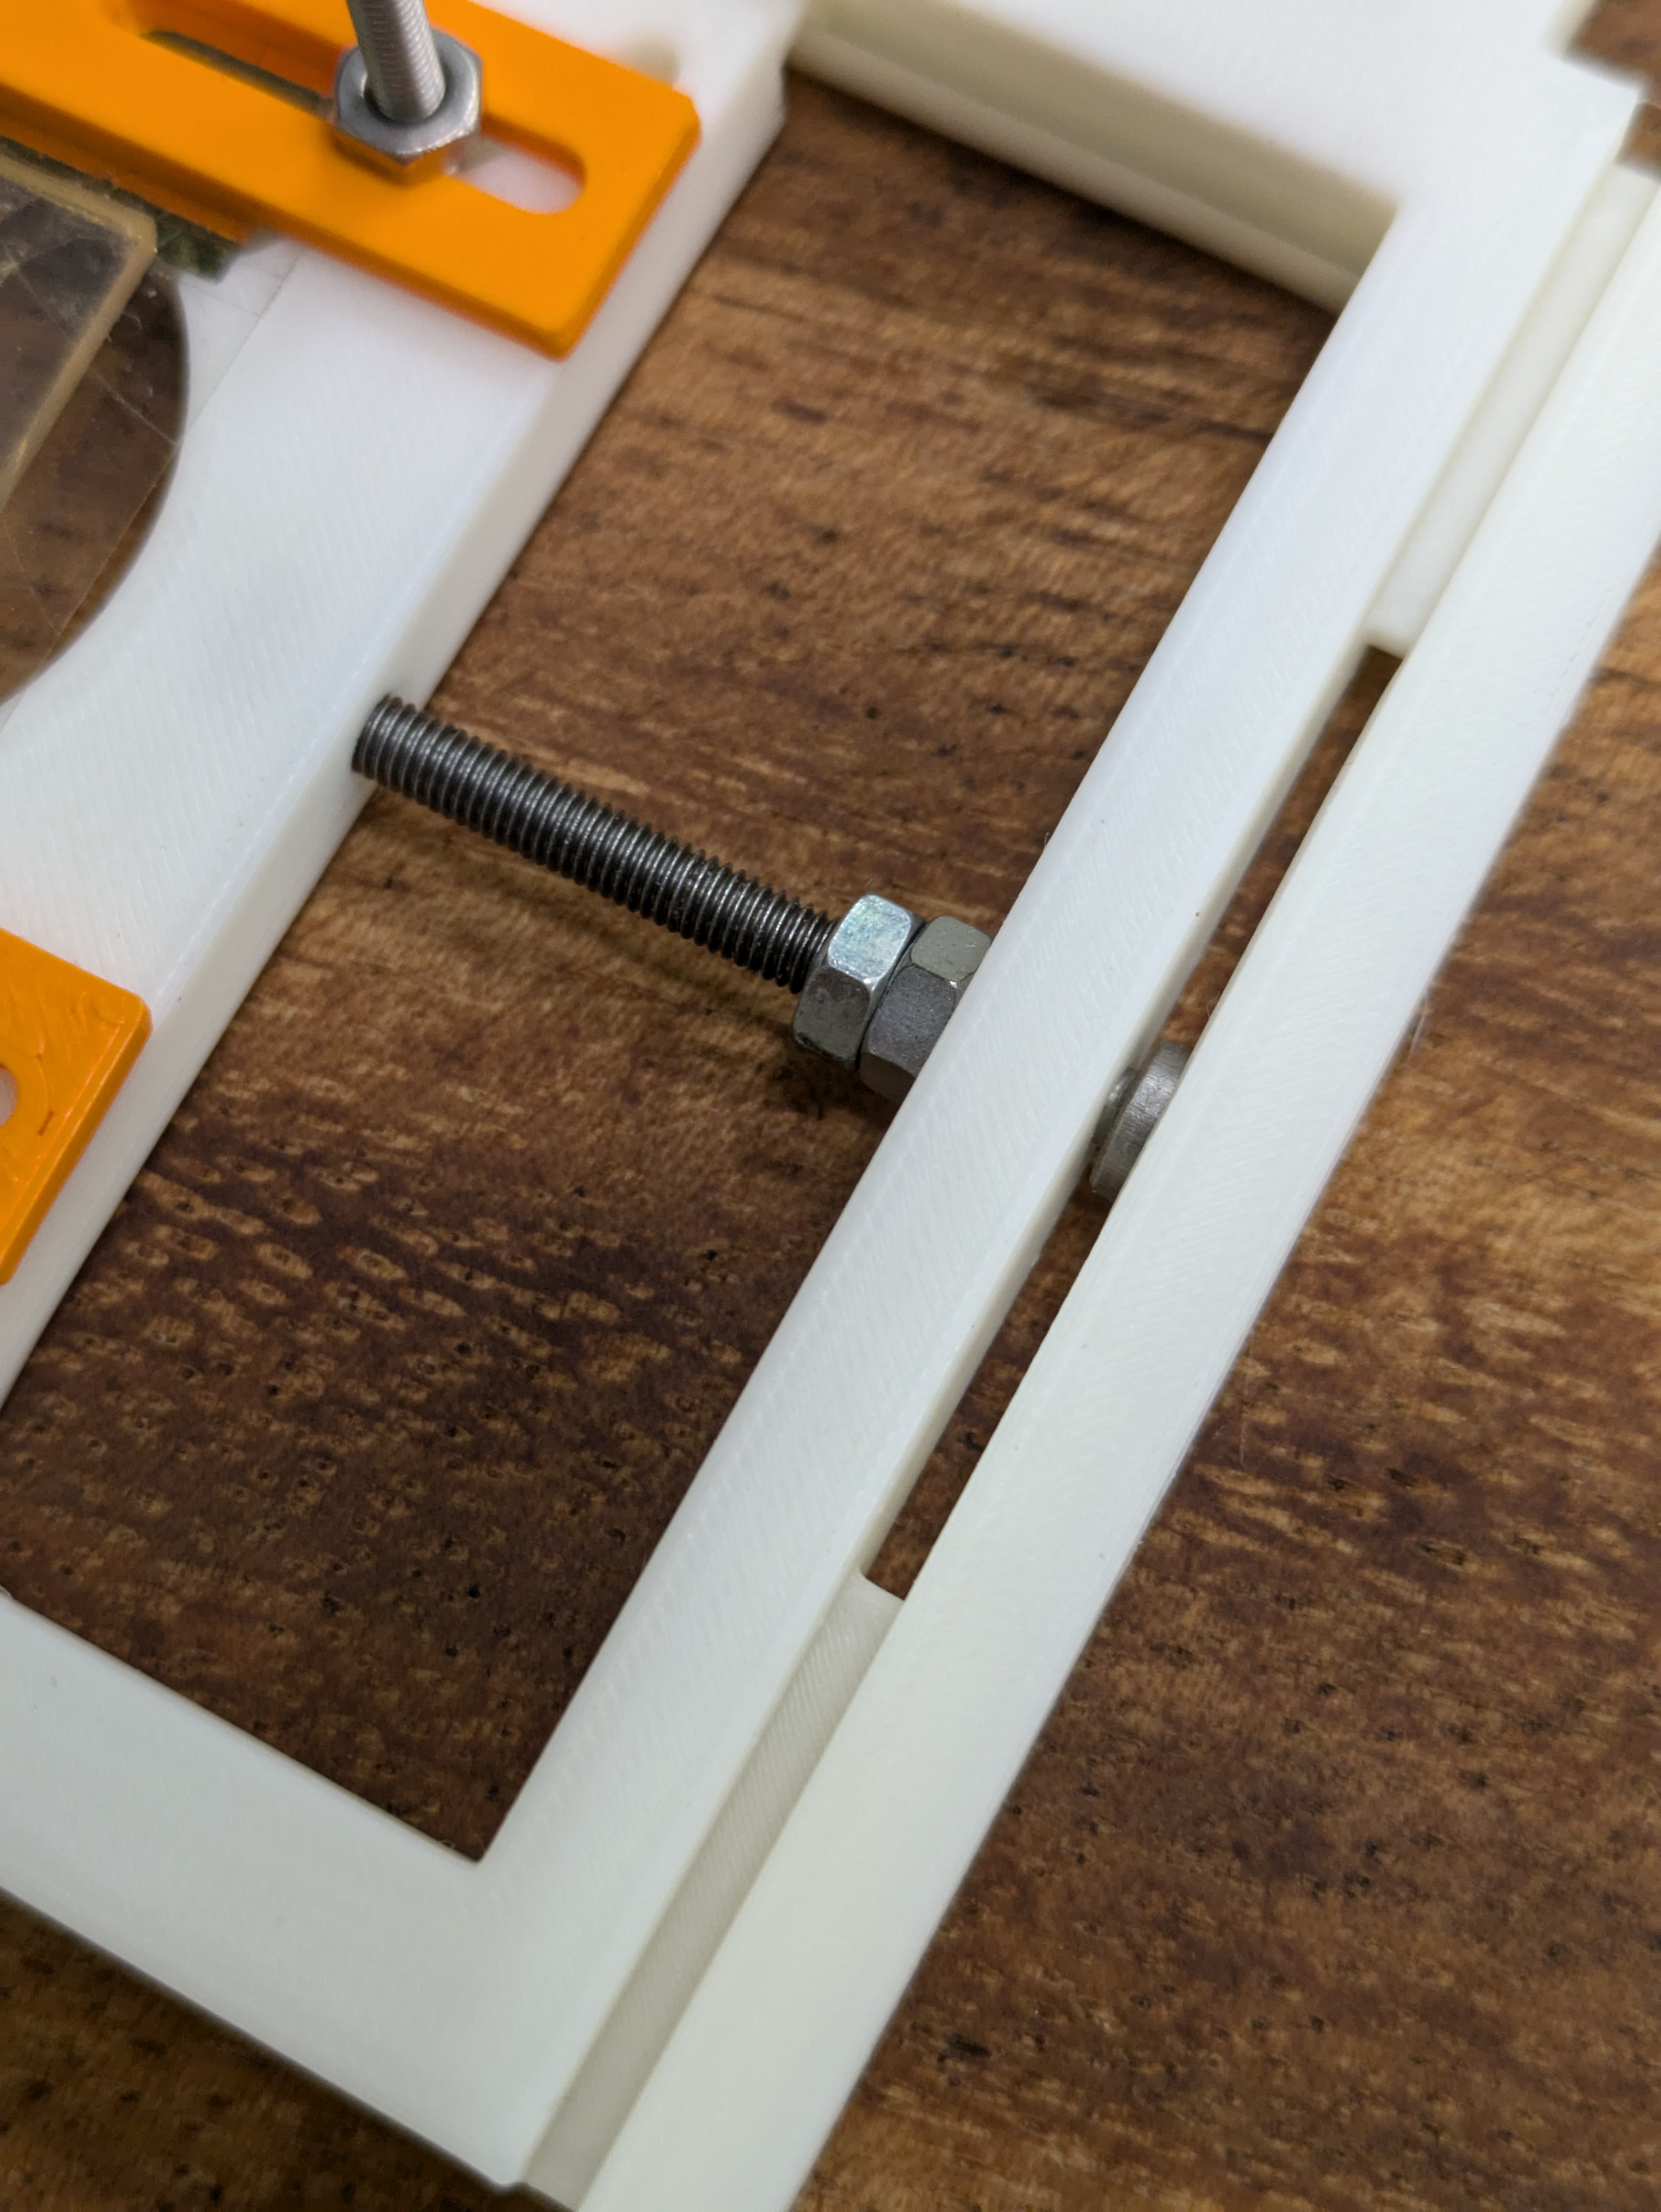
\includegraphics[width=\textwidth]{images/side_nut.jpg} 
        \caption{Properly Installed Side Nut }
    \end{minipage}
\end{figure}

Lastly, in order to later install the plaques securing the sample to the sample holder, slide the four M2.5 bolts in the cavities in the center of the sample holder, see figure 2 for the cavities.

\section*{Sample Securing Plaques}

In order to ensure that the sample does not move around as the sample holder is moved, we have designed two plaques that can be held in place by threading the four M2.5 nuts into the bolts that were previosuly inserted in the stage, as 
shown in figure 8.


\begin{figure}[h!]

\end{figure}

\begin{figure}[h]
    \centering
    \begin{minipage}[b]{0.45\textwidth}
    \centering
    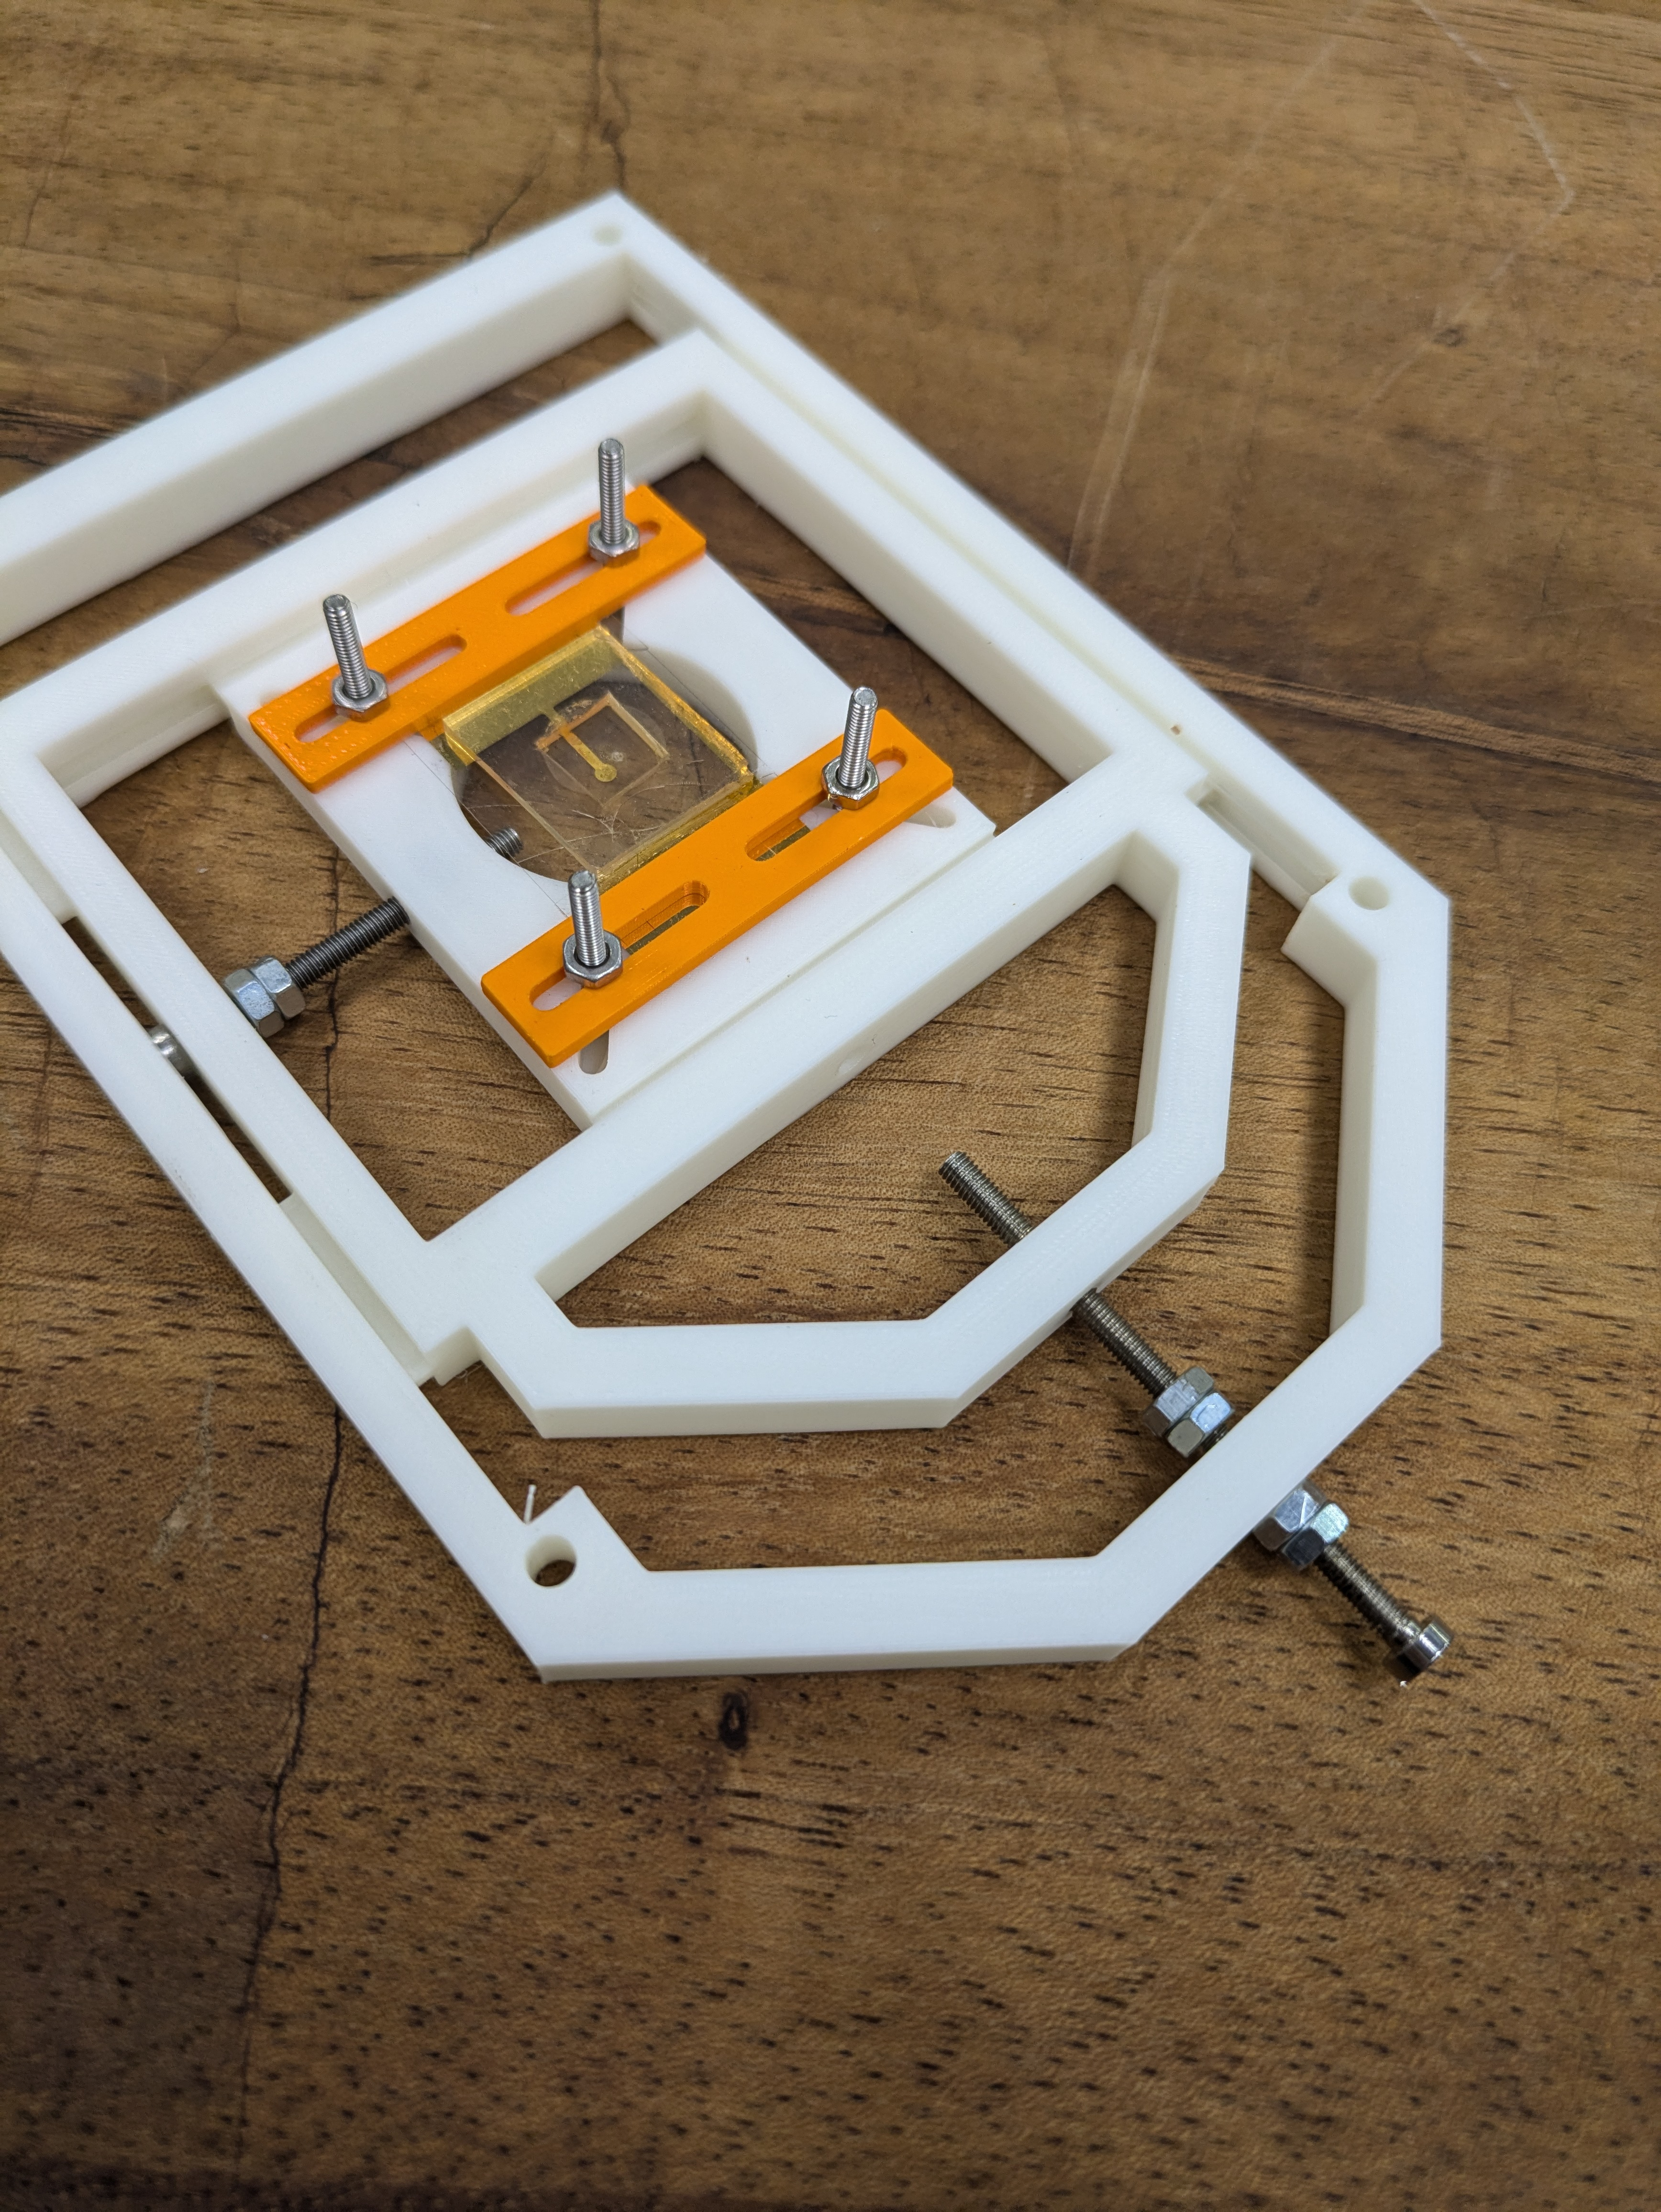
\includegraphics[width=\linewidth]{images/slide_holder_complete.jpg}
    \end{minipage}
    \hfill
    \begin{minipage}[b]{0.45\textwidth}
    \centering
    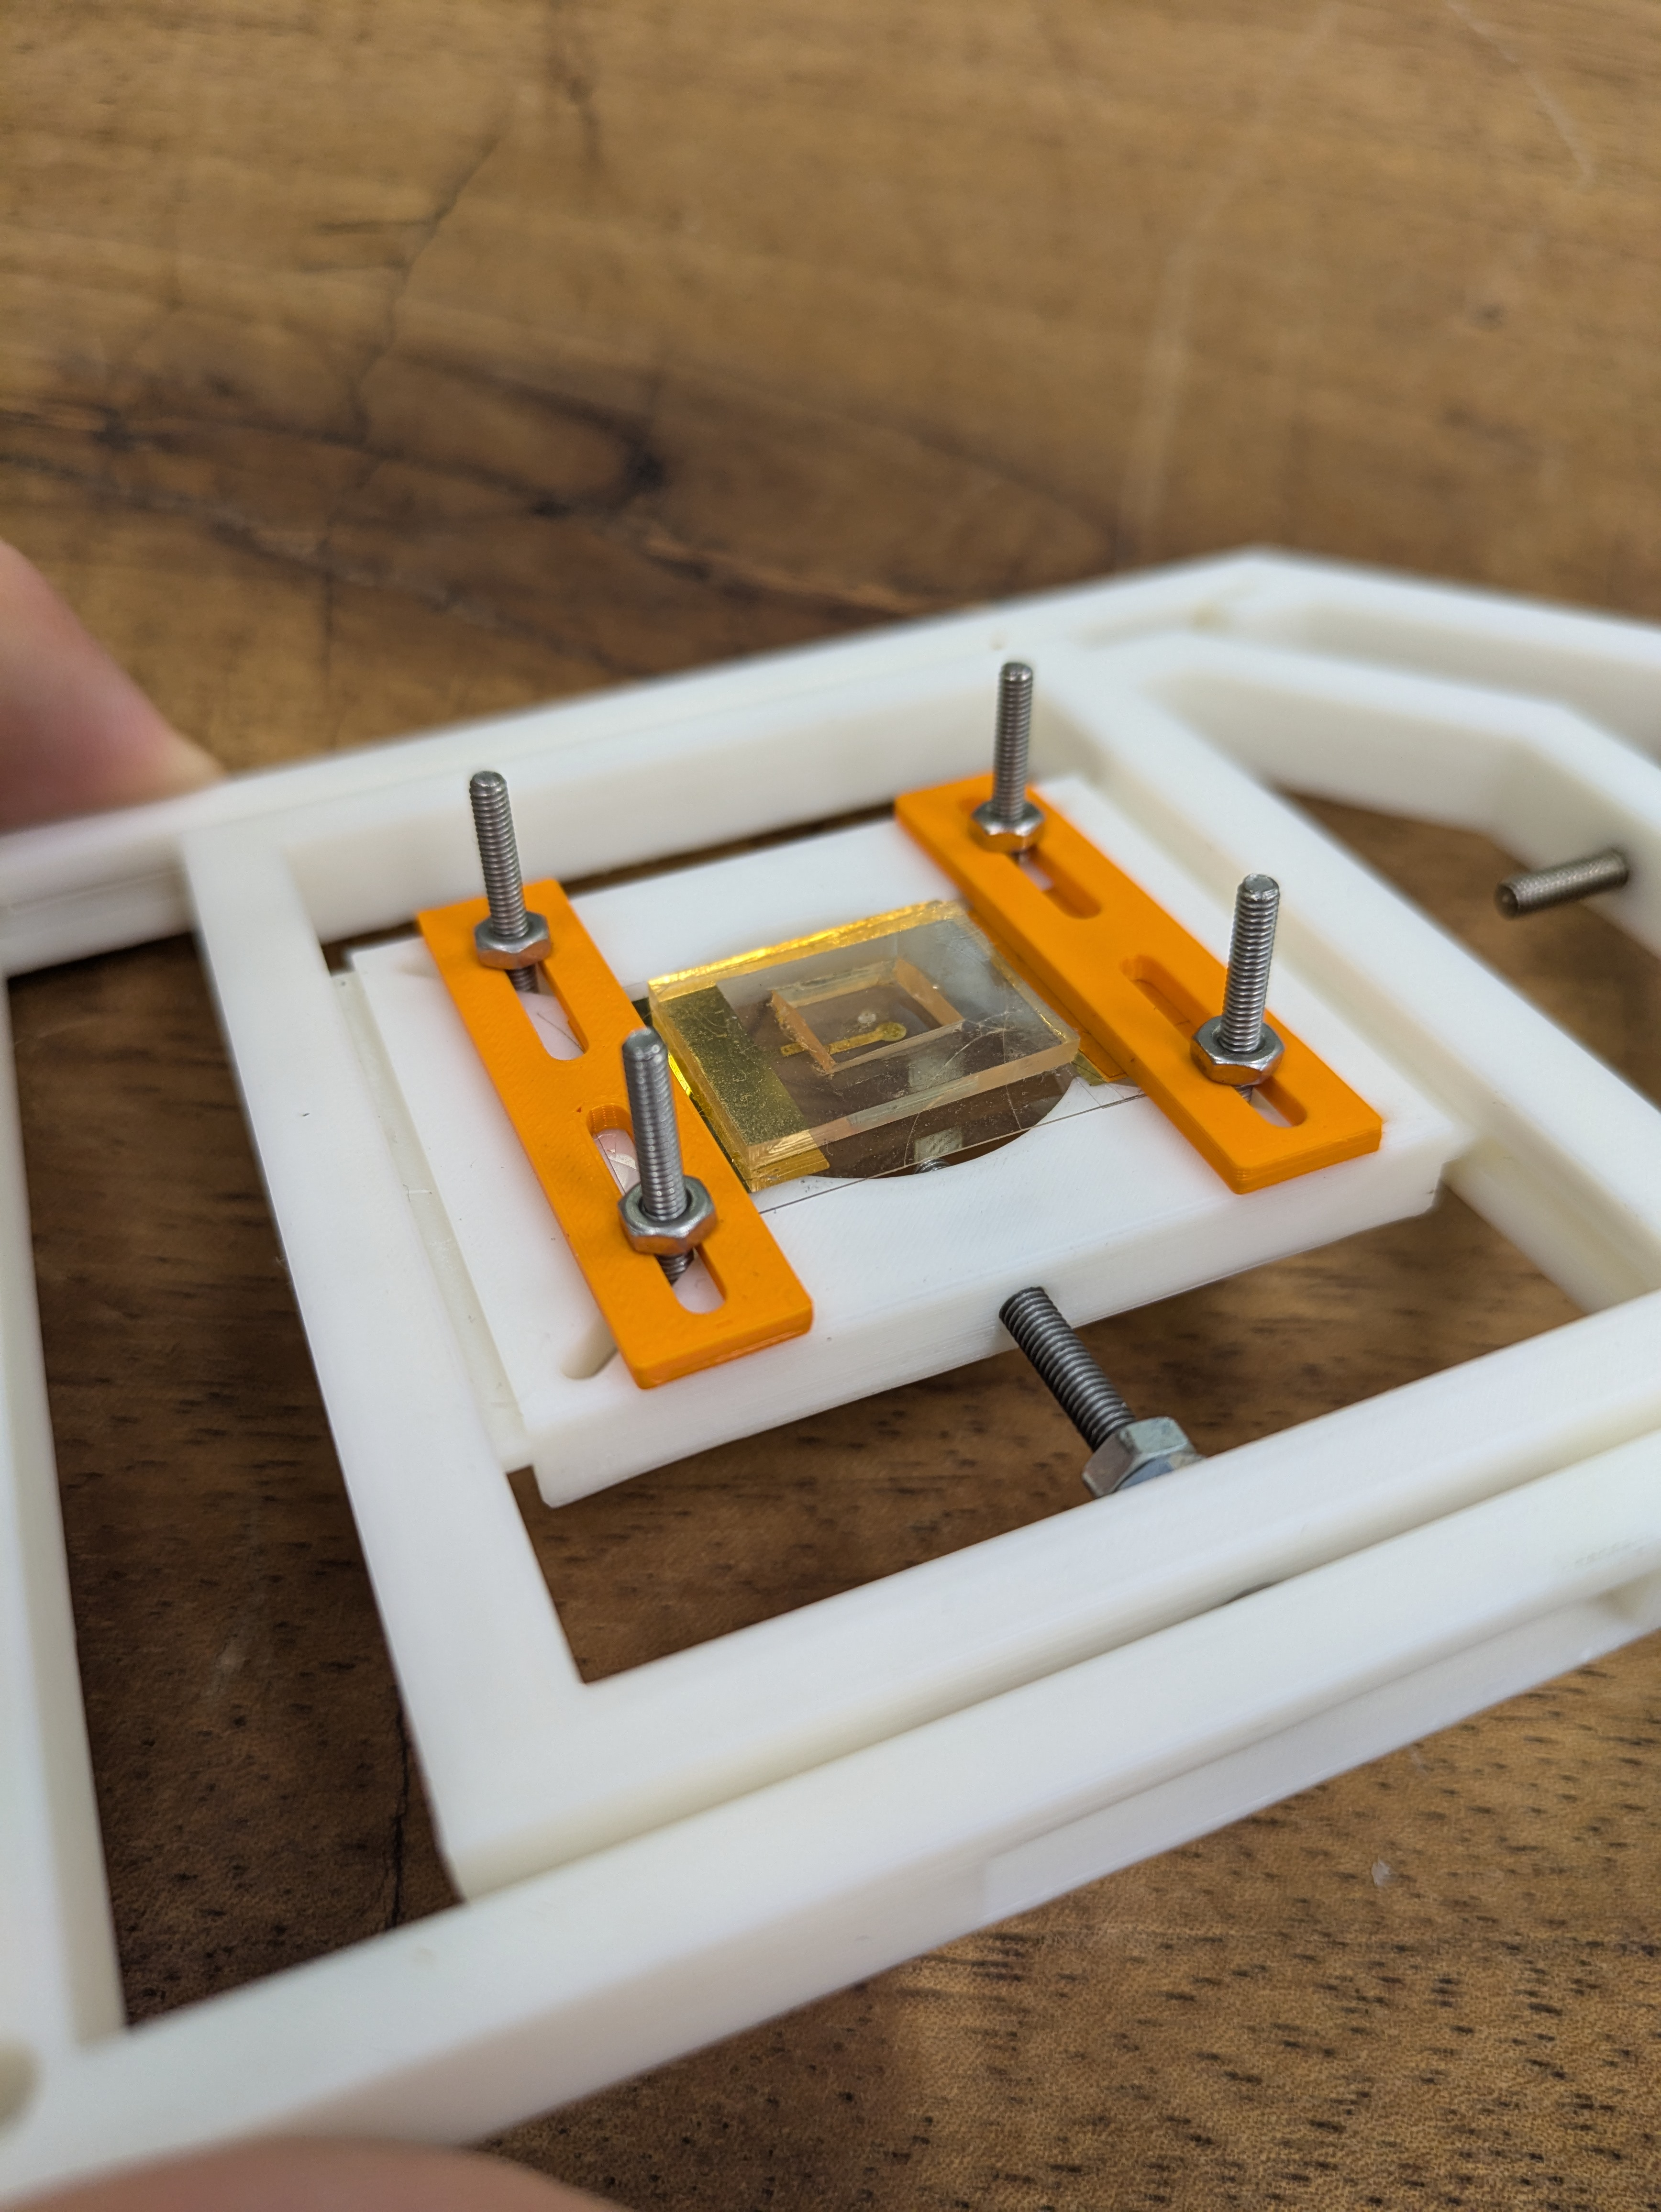
\includegraphics[width=\linewidth]{images/slide_holder_complete1.jpg}
    \end{minipage}
    \caption{Complete Sample Holder with Plaques}
\end{figure}


The plaques should be printed with a 15\% infill. The design file for the plauqes is found under plaques.f3d. 

\end{document}
